\documentclass[a4paper, 12pt]{article}
\usepackage{t1enc}
\usepackage[utf8]{inputenc}
\usepackage[english, magyar]{babel}
\usepackage{graphicx}
%\usepackage{times}
\usepackage{hyperref}
\hypersetup{
	colorlinks,
    citecolor=black,
    filecolor=black,
    linkcolor=black,
    urlcolor=black
}
%hivatkozások feketék legyenek
\usepackage{url}
\def\UrlBreaks{\do\/\do-}
%megtörheti az urleket a / és a - karaktereknél
%\usepackage{sidecap}
%\usepackage{glossaries}
\sloppy
\frenchspacing
\usepackage{geometry}
\geometry{margin=2.5cm}
\usepackage{textcomp} %~ hullám miatt
\usepackage{float} %ábrákhoz
\usepackage{pdfpages}
\usepackage{pifont}
\newcommand{\cmark}{\ding{51}}%
\newcommand{\xmark}{\ding{55}}%
\usepackage[binary-units=true]{siunitx}

\newcommand{\tab}{\hspace*{1em}}

\renewcommand*{\thefootnote}{(\arabic{footnote})}



\begin{document}
%
\includepdf{DiptervFeladatkiiras.pdf}
%\pagestyle{plain}
\begin{titlepage}
\begin{center}

\includegraphics[width=60mm,keepaspectratio]{bme}\\
\vspace{0.3cm}
\textbf{Budapesti Műszaki és Gazdaságtudományi Egyetem}\\
\textmd{Villamosmérnöki és Informatikai Kar}\\
\textmd{Automatizálási és Alkalmazott Informatikai Tanszék}\\[5cm]

\vspace{0.4cm}
{\huge \bfseries Vezérlőegységek automatizált tesztelésére, programozására és kalibrálására
szolgáló berendezés tervezése és megvalósítása}\\[0.8cm]
\vspace{0.5cm}
\textsc{\Large Diplomaterv}\\[4cm]


\begin{tabular}{ccc}
 \makebox[5cm]{Budavári Ruben Pál} & \makebox[5cm]{Dr. Iváncsy Szabolcs} & \makebox[5cm] {Banai András}\\
 \makebox[5cm]{\emph{Készítette}} & \makebox[5cm]{\emph{Egyetemi konzulens}} & \makebox[5cm]{\emph{Külső konzulens}}
\end{tabular}
\vfill
{\large \today}
%{\large \date{2017. május 06.}}
\end{center}
\date{2016. 06. 06.}
\setcounter{page}{1}
\end{titlepage}

%--------------------------------------------------------------------------------------
% Tartalomjegyzék
%--------------------------------------------------------------------------------------
\tableofcontents
\clearpage


%--------------------------------------------------------------------------------------
% Nyilatkozat
%--------------------------------------------------------------------------------------
\begin{center}
\large
\textbf{HALLGATÓI NYILATKOZAT}\\
\end{center}

Alulírott Budavári Ruben Pál, hallgató kijelentem, hogy ezt a diplomatervet meg nem engedett segítség nélkül, saját magam készítettem, csak a megadott forrásokat (szakirodalom, eszközök stb.) használtam fel. Minden olyan részt, melyet szó szerint, vagy azonos értelemben, de átfogalmazva más forrásból átvettem, egyértelműen, a forrás megadásával megjelöltem.

Hozzájárulok, hogy a jelen munkám alapadatait (szerző(k), cím, angol és magyar nyelvű tartalmi kivonat, készítés éve, konzulens(ek) neve) a BME VIK nyilvánosan hozzáférhető elektronikus formában, a munka teljes szövegét pedig az egyetem belső hálózatán keresztül (vagy autentikált felhasználók számára) közzétegye. Kijelentem, hogy a benyújtott munka és annak elektronikus verziója megegyezik. Dékáni engedéllyel titkosított diplomatervek esetén a dolgozat szövege csak 3 év eltelte után válik hozzáférhetővé.

\begin{flushleft}
\vspace*{1cm}
Budapest, \today
\end{flushleft}

\begin{flushright}
 \vspace*{1cm}
 \makebox[7cm]{\rule{6cm}{.4pt}}\\
 \makebox[7cm]{hallgató}
\end{flushright}


\thispagestyle{empty} %nincs oldalszám
\vfill
\clearpage

%--------------------------------------------------------------------------------------
% Összefoglaló
%--------------------------------------------------------------------------------------
\selectlanguage{magyar}
\section*{Összefoglaló}
A diplomamunkám során a Leviathan Solutions Elektronikai és Fejlesztő Kft. által fejlesztett beléptető- és munkaidő-nyilvántartó rendszer részét képező mikrokontrolleres panelhez terveztem egy tesztelő berendezést. A mikrokontrolleres panel feladata az ajtóknál elhelyezett olvasóktól érkező adat feldolgozása és a jogosultságoknak megfelelő reagálás, például ajtónyitás vagy visszajelző relé meghúzása. A megtervezendő eszköz feladata, hogy kapcsolódjon a kontrolleres panel (ezután ACU) be- és kimeneteire, ellenőrizze, hogy azokon nincs-e rövidzár és hogy funkcionálisan is megfelelően működnek-e. A termékcsaládhoz tartozik egy táppanel is, ennek a kalibrációja során többféle feszültséget és terhelést kéne manuálisan kapcsolni az eszközre. A teszternek feladata ezt a folyamatot is automatizálni. A diplomamunkám során megterveztem a teszter kapcsolási rajzát, valamint pcb tervét és megírásra került hozzá a firmware is. A firmware-nek tudnia kell parancsokat és adatokat fogadnia ethernet kapcsolaton keresztül és ennek megfelelően tesztet futtania; ami lehet rövidzárteszt, táppanel kalibráció vagy akár tesztadat szimulálása is, ami során ellenőrizzük, hogy megtörténik-e a megfelelő válasz az ACU részéről.


\thispagestyle{empty} %nincs oldalszám
\clearpage

%--------------------------------------------------------------------------------------
% Abstract
%--------------------------------------------------------------------------------------
\selectlanguage{english}
\begin{otherlanguage}{english}

\section*{Abstract}


\end{otherlanguage}
\thispagestyle{empty} %nincs oldalszám
\clearpage

\selectlanguage{magyar}

\section{Bevezetés}
\tab A diplomamunkám során első lépés volt megismerni a beléptetőrendszert és átbeszélnünk, hogy pontosan milyen teszteket szeretnénk elvégezni. Mivel jelenleg is több ACU van használatban és ezeknek a meghibásodása esetén szeretnénk megtudni, hogy mi okozta a hibát; valamint a legyártott eszközöknél jó lenne elleőriznünk, hogy jó lett-e mindenhol a beforrasztás és sikeres volt-e a firmware-feltöltés, ezért célszerű egy olyan eszköz, ami ezeket elvégzi automatikusan vagy csak minimális emberi beavatkozással. Sok óra munkát meg tudunk azzal spórolni, ha ezek a tesztek konzisztensen, gyorsan és minimális felügyelettel elvégezhetőek. Ezen felül automatikus tesztek futtatására is használható a teszter, például bizonyos események generálására adott válasszal kell, hogy reagáljon a készülék. Az átbeszéltek alapján szükség van egy rövidzártesztre, ekkor még nem indítjuk el az ACU-t (nem adunk neki tápfeszültséget), hanem vizsgáljuk, hogy a kritikus pontokon nincs-e rövidzár. Második teszt futtattása, amikor elindítjuk az eszközt és megnézzük, hogy feléled-e. Ha van rajta firmware, akkor azt ellenőrithetjük is a megfelelő bemenetekre adott megfelelő jelekkel. A teszter feladata, hogy a bootloader és a firmware feltöltését az ACU-ra megkönnyítse. \\
A diplomamunkámat egy félévnyi önálló laboratóriumi munka előzte meg\footnote{az önálló laboratóriumi beszámolóból átemelt részek dőlt betűvel szerepelnek ebben a dolgozatban}, amiben elkészült a teszternek egy terve. Ezt a tervet több okból át kellett alakítani, amik közül az egyik volt, hogy szeretnénk, ha a termékhez tartozó táppanel kalibrációját is meg lehetne gyorsítani, ami jelenleg körülbelül 8-10 percet vesz igénybe és folyamatos emberi beavatkozást igényel. Ehhez a kalibrációhoz 8V és 13.8V között változtatható feszültségre van szükségünk, ami maximum 6A-ig terhelhető, valamint különböző terheléseket kell kalcsolni a táppanelre, miközben az kalibrálja magát és soros porton kommunikál a teszterrel. Ahhoz, hogy teljesen értsük milyen feladatokat kell megvalósítanunk, először meg kell értenünk a rendszer működését.
\subsection{Beléptetőrendszer bemutatása}
\tab A beléptető két részből áll, egyik a PC-s szoftver, ahol a jogosultságokat lehet kiadni, embereket lehet regisztrálni és különböző feltételeket lehet szabni, ami alapján eldöntjük, hogy ki hova mehet be, mikor szeretnénk kameraképet látni a képernyőn vagy akár lekérdezhetünk munkaidőriportokat. Ez a szoftver etherneten kommunikál az ACU-kkal, amiből elméletileg akármennyi lehet egy rendszerben.\\
Minket a másik egység érdekel, ez egy mikrokontrolleres panel (ACU), ami az ajtók vezérlését végzi. Egyszerre 4 olvasót tud kezelni, ezek lehetnek PIN-es vagy kártyás beléptetők. Ezek az olvasó berendezések Wiegand kapcsolaton kommunikálnak a panelünkkel, ami egy kétvezetékes, párszor 10kHz-es protokoll. 4 relével az ajtókat tudja nyitni vagy csukni. Ki tudjuk választani jumperekkel, hogy 12V és GND között kapcsoljon vagy szárazkontakttal jelezzük az ajtó nyitását/zárását, ez utóbbi esetben kívülről kell a kívánt feszültségjelet biztosítanunk, amit egy másik vonalon kapcsol az eszköz. Alapkonfigurációban az ACU-hoz négy ajtó és mindegyikhez egy-egy olvasó, valamint nyomógomb tartozik. Ezt szoftverből át lehet állítani, így egytől négy ajtóig bármit beállíthatunk és ha kevesebb, mint 4 ajtóval dolgozunk, akkor a felszabaduló olvasóbemeneteket használhatjuk valamelyik másik ajtóhoz a másik irány vezérlésére. Ezeknek az ajtóknak 5 típusa van:
\begin{itemize}
\vspace{-0.4em}
\item  Lehetnek normális ajtók, ekkor az olvastatás után előre beállított ideig nyitott állapotba kerül az ajtó, ekkor át lehet menni, ez idő lejárta után pedig becsukódik.
%\vspace{-0.5em}
\item Másik lehetőség a bistabil ajtó. Ebben az esetben az érvényes kártyaolvastatás vagy pin beütése az ajtó nyitottságát megváltoztatja és úgy hagyja a következő érvényes olvastatásig.
\vspace{-0.5em}
\item Harmadik lehetőség a forgóvilla. Ebben az esetben mindenképpen két ajtórelét fel kell használnunk egy forgóvillához a két irány miatt. Ezeket az eszközöket csak egy-egy nyitóimpulzussal vezéreljük.
\vspace{-0.5em}
\item Negyedik és ötödik lehetőség a kapu és a sorompó, ezek vezérlésükben leginkább a normális ajtókhoz hasonlítanak, őket is előre beállított ideig tartjuk nyitott állapotban, aztán visszazárnak.
\vspace{-0.5em}
\end{itemize}
Emellett mind a 4 olvasóhoz tartozik nyomógombos bemenet is, mert sok helyen csak a befelé irányban kell azonosítani magunkat, kifelé elég gombot nyomnunk. Minden ajtóhoz alkalmazhatunk nyitásérzékelőt is, ezeknek kétféle működése van: Egyik megoldás, hogy amikor kinyílik az ajtó fizikailag, egyből visszazár a relé, így az visszacsukás után nem nyitható újra. Másik lehetőség, hogy amíg az ajtó nyitási ideje tart, addig húzva tartjuk a relét, tehát ez idő alatt többször is ki lehet nyitni az ajtót. Minden olvasóhoz beköthető két ledvisszajelzés és egy beep. Ezek a kártyát olvastató felhasználó számára adnak visszajelzést, ami lehet érvényes vagy érvénytelen olvastatás jelzése, táskaellenőrzés feltartóztatás riasztása és még számos visszajelzés.\\
Az eszközben elérhető 2-2 AUX be- és kimenet. Ezekre rengeteg funkciót lehet vezetni. Jelezhetjük itt a ``Ne zavarjanak'' igényünket, használható ajtónyitás követésére, periódikus jelzésre, véletlenszerű kapcsolásra adott százalékkal, \dots A berendezés megbontását észlelendő egy bemenet áll rendelkezésünkre, továbbá van egy FIRE bemenet, ami kinyitja az összes ajtót beállítástól függetlenül, ez lehet NO vagy NC is, jumperrel választható.\\
Az ACU és a PC-s szoftver folyamatos kapcsolatban van egymással, minden történésről eseményt generál és elküldi a szoftvernek az eszköz, valamint globális funkciók\footnote{Olyan funkciók, amiben több kontroller egyszerre vesz részt, ekkor a PC-s szoftver hozza meg a döntést, hogy kinyithatja-e az adott illető az ajtót. Ilyen lehet például egy létszámkorlát, amiben 2-3 kontroller is ugyanahhoz a területhez tartozik.} esetén lekérdezi a jogosultságokat.

\subsection{Célok és tesztelő berendezés}
\tab A feladat, hogy ehhez a vezérlőegységhez egy tesztert készítsünk, amivel az esetleges rövidzárakat tudjuk megtalálni a fontosabb helyeken; a rendeltetésszerű működést tudjuk ellenőrizni; teszteseteket tudunk generálni (például egy kártyaolvastatást) és eközben folyamatos kapcsolatban állunk egy számítógéppel, ami felügyeli a tesztelést és szükség esetén utasításokat lehet kiadni rajta keresztül. A másik feladat, a korábban említett táppanel kalibrációjának meggyorsítása. Az egyértelmű szóhasználat miatt a \emph{vezérlőegység, kontrolleres panel, ACU} lesz a beléptetőrendszerhez tartozó panel és \emph{teszter}, amit tervezünk.\\
A fentebb említett üzemmódok részletesebben:
\begin{enumerate}
\item \underline{Rövidzárteszt:} A vezérlőegység tápfeszültség nélküli tesztelése, ekkor a ki- és bemeneti, valamint tápvonalakat ellenőrizzük, hogy nincs-e valahol rövidzár.
\item \underline{Alap teszt és felprogramozás:} A vezérlőegységre tápfeszültséget kapcsolva ellenőrizzük, hogy a megfelelő helyeken megvannak-e a tápfeszültségek és az értékük is jó-e, ezért ez utóbbi a méréseket ADC-vel végezzük. Ha kontroller nem volt még használva, akkor először bootloadert kell rá tölteni. Két ATxmega mikrovezérlő található egy panelen, amiket a PDI bemenetükön lehet programozni. Hogy ez gyorsan menjen, ezért nekünk kell megoldanunk, hogy a programozót ne kelljen manuálisan átdugdosni, hanem egy analóg switch-csel fogjuk kapcsolni a vonalakat. A bootloader után már Etherneten tudja fogadni a normál firmware-t az eszköz.
\item \underline{Tesztadatos tesztelés:}Ha már felprogramozták az eszközt, akkor az alapvető funkcionális tesztek elvégezhetőek rajta miután néhány alapbeállítást feltöltünk rá (például, hány ajtó legyen, néhány tesztfelhasználó, \dots). A tesztadatok feltöltése után nézzük, hogy bizonyos bemenetekre, az azoknak megfelelő választ adja-e, jó ajtót nyit ki, jó ledet villant fel, jó időben teszi mindezt, a feszültségek közben hogyan változnak, \dots
\item \underline{Táppanel kalibráció:} A táppanelre a firmware feltöltése (szintén PDI) után 8V és 13.8V közötti feszültségeket kell kiadni 5-6 lépésben, amiben kell lennie egy elég pontos 12V-nak. Ezután kell 12\si{\ohm}-ot és 2.5\si{\ohm}-ot kapcsolni terhelésként az 1A-es és az 5A-es ágra. A teszt alatt UART-on kommunikálunk a táppanellel, és jelezzük, hogy milyen értékeket kellett mérnie az adott beállításnál.
\end{enumerate}

\section{Mérendő jelek}
\tab A lentebbi táblázatban [\ref{merendojelek} .táblázat] láthatóak a vezérlőegység jelei, amiket szeretnénk valamilyen módon mérni vagy generálni:

\begin{table}[H]
\caption{Mérendő és generált jelek}
\center
\label{merendojelek}
\begin{tabular}{p{4cm}|p{6cm}|p{0.5cm}|p{0.5cm}|p{0.5cm}|p{1cm}}
\hline
Jel & Megjegyzés & \rotatebox{90}{Mennyi van belőle} & \rotatebox{90}{Rövidzárteszt} & \rotatebox{90}{Mi generáljuk} & \rotatebox{90}{Mérjük}\\
\hline
Olvasó Wiegand jele & D+ és D- jel & 4x2 & \cmark & \cmark & \xmark\\
\hline
Olvasók ledjei & Ezzel adunk visszajelzést az olvasóknak. & 4x2 & \cmark & \xmark & \cmark\\
\hline
Olvasók ``beep'' jelei & Az olvasóba épített hangszórót vezérli. & 4 & \cmark & \xmark & \cmark\\
\hline
Ajtónyitógombok & & 4 & \cmark & \cmark & \xmark\\
\hline
Nyitásérzékelők & & 4 & \cmark & \cmark & \xmark\\
\hline
Ajtónyitó relék & NO és NC vonal is. Ellenállásosztóval mérjük.& 4x2 & \xmark & \xmark & \cmark\\
\hline
EM & Vészhelyzet gomb bemenete. & 4 & \xmark & \cmark & \cmark\\
\hline
FIRE & Tűzjelző bemenet. & 1 & \cmark & \cmark & \xmark\\
\hline
TMP & Megbontásérzékelő. & 1 & \cmark & \cmark & \xmark\\
\hline
AUX bemenetek & A teszter felől nézve kimenet. & 2 & \cmark & \cmark & \xmark\\
\hline
AUX kimenetek & A vezérlőegység felől kimenet. NO és NC vonal.& 2x2 & \cmark & \xmark & \cmark\\
\hline
Ethernet & RJ45 csatlakozón keresztül. & 1 & \xmark & \cmark & \cmark\\
\hline
Tápfeszültségek.& 12V, 3.3V, akkumulátor töltőfeszültség & 3 & \cmark & \xmark & \cmark\\
\hline
1Hz & A vezérlőegység RTC-je által szolgáltatott 1 Hz-es jel. & 1 & \xmark & \xmark & \cmark\\
\end{tabular}
\end{table}


\section{Hardver}
\subsection{Alkatrészek kiválasztása}
\tab A teszter egy mikrokontrolleres panel lesz, ami egy tűágyhoz kapcsolódik. A tűágyba helyezzük a vezérlőegységet és így tudunk hozzá kapcsolódni. A tűágyhoz a teszter 2 db 40-es IDC csatlakozóval és a hozzájuk tartozó szalagkábelekkel fog csatlakozni.

\subsubsection{Mikrokontroller}
\tab A mikrokontroller kiválasztásánál először meg kell határoznunk, hogy milyen funkciókat kell biztosítson ahhoz, hogy a kitalált feladatot el tudja látni. Az alábbi szempontok voltak a mérvadóak a döntésünkben.
\begin{itemize}
\item Megfelelő számú GPIO port, amivel tudunk kapcsolódni az ACUhoz és a külső IC-khez, kapcsolásokhoz.
\item Támogassa hardveresen a megfelelő kommunikációs protokollokat, amire szükségünk lesz:SPI, UART.
\item 3.3Vról működjön. Erre azért van szükség, mert a kontrolleres panel is és a táppanel is 3.3V-ról működik, így nem kell a szintillesztéssel foglalkozni.
\item Legyen AD átalakító benne, mert szükséges a tápfeszültségeket mérni és ha megoldható, akkor ezt belső AD-vel tegyük.
\item Ingyenes fejlesztői környezet.
\item[-] Nem elsődleges, de figyelembe vett szempontok voltak még:
\item Legyen hozzá fejlesztőpanel, így a firmware írását már akkor el lehet kezdeni, amikor még nem került legyártásra a panel.
\item Ha van olyan mikrovezérlő, amit már használtak/használnak a cégen belül, akkor tudnak tapasztalattal segíteni a kollegák.
\item Legyen benne a sok funkciók miatt elegendő flash és ram, így nem kell külsőt használni. Mindekettőből párszor 100kB már elegendő.
\item Támogassa az Etherneten való kommunikációt, például TCP/IP stack-kel vagy akár a fizikai réteg meglétével.
\end{itemize}
\tab Így esett a választás a Texas Instruments TM4C1294NCPDT\textregistered{} \cite{tm4c} mikrokontrollerére. Felületszerelt, 128 láb, ebből 90 GPIO és ezen felül vannak az Ethernet vonalak, a kiválasztott protokollokat támogatja (4 SPI, 8 UART, ezek a 90 GPIO vonal között vannak), Ethernet MAC és PHY integrálva, 20 AD csatorna, 1MB Flash memória és 256 kB SRAM. Ha a fentebbi táblázatot megnézzük, látjuk, hogy szükséges ha mindegyik vizsgált jelre csak egy GPIO vonalat használunk el, az is 50 láb és erre jön rá a többi funkció (UART, saját ledek, nyomógomb, \dots)

TODO ethernet miatt 25MHz kristály
TODO fejlesztőpanel + kép


\subsubsection{GPIO bővítőmodul}
\emph{
\tab Annak ellenére, hogy a mikrokontrollernek 128 lába van, még ez sem elég ahhoz, hogy az összes ki- és bemeneti jelet tudja kezelni, ezért szükséges volt valamilyen módon bővíteni a GPIO lábakat. A Microchip\textregistered{} gyárt SPI-os és I2C-s GPIO bővítőmodulokat is, 8 és 16 GPIO lábbal. Ezek átlagos IO lábakként működnek (ki és bemenetként is használhatóak, felhúzóellenállás kapcsolható a lábakra, amit egyenként lehet állítani, interruptot is tudnak generálni szintre vagy élre). 2 db 16 lábas (MCP23S18) \cite{mcp23s18} SPI-os chipet választottam.\\
SPI-on 10MHz-cel tudunk kommunikálni, ezzel a lassabban változó jeleket bőven tudjuk kezelni. Ezek a ledek, beep jelek, nyomógombok, nyitásérzékelők, ajtónyitó kimenetek. Az eszközök 2-2 interrupt vonalon tudnak jelezni a mikrokontrollerünk felé, ha változás történik; az IC lábai két portba vannak rendezve, ezzel szétválasztva és megkönnyítve a kezelést.}


\subsubsection{Flash}
\tab Bár a mikrokontrollerünkben található 1MB flash-t valószínű nem fogjuk teljesen kihasználni, mégis szükséges egy külső adattároló is, mivel teszteseteket kell tárolnunk és igény esetén kell tárolnunk az ACU formware-ét is, ami mi magunk fogunk feltölteni rá. Ehhez AT45DB641 \cite{flash} típusú 32MB-os flasht választottam. Ennek külön előnye, hogy van egy 256 byte-os SRAM benne (ez megegyezik a page mérettel), így támogatni tudja a\emph{read-modify-write} parancsot, aminek köszönhetően ha szeretnénk egy adatot módosítani, akkor nem kell kiolvasnunk az azon page-en levő összes adatot, törölni a lapot és újra beírni, hanem elegendő az úja adatot leküldeni a tárolónak és az a saját bufferén keresztül ezt belül elintézi. SPI protokollal tudunk kommunikálni az eszközzel.

\subsubsection{3.3V-os táp}
\tab A 3.3V-os vonalunkon van az összes IC, ezért ennek az összes fogyasztása extrém esetben elérheti a 600mA-t is. Ez az az eset, amikor minden eszköz a maximumot fogyasztja, amit csak lehet; normál működés közben ez nem fordulhat elő, de ha nagyobb terhelésre tervezzük a tápot, azzal baj nem lehet. Mivel 12V-ot használnunk kell a teszterben bizonyos kimeneti tranzisztorokhoz ezért célszerűen 12V-os bemeneti tápot használunk az egész teszter működéséhez és ebből állítjuk elő, a nekünk szükséges 3.3V-ot. Sima LDO használata esetén sok energia elveszne a nagy feszültségesés és nagy áram miatti teljesítményben, ezért döntöttem a kapcsolóüzemű DC/DC átalakító mellett. Ezek közül egy jól használható az MC34063AD \cite{dcdc} DC-DC konverter, amihez számos online elérhető kalkulátort hívhatok segítségül, hogy a tervezett feszültség és áramértékek mellett meg tudjam határozni a többi alkatrész (ellenállás, kondenzátor, tekercs) nagyságát. Én \emph{\href{http://www.bobtech.ro/tutoriale/componente-electronice/43-calculator-online-mc34063a-mc34063-step-down-step-up-inverter}{ezen a linken}} elérhető oldalt használtam erre.
Figyelnünk kell rá, hogy a bemeneten levő ellenállás ne csak értékileg legyen jó, hanem ki is bírja ezt a terhelést, ezért legalább 0.4W-os ellenállást kellett ide választanunk.

\subsubsection{Analóg switch a programozáshoz}
\tab PDI programozón keresztül fogjuk a kontrolleres paneleket programozni, és ahhoz, hogy ne kézzel kelljen átdugni a programozót egy analóg switch-es kapcsolást választottam. Maga a programozó egy PC-hez lesz csatlakoztatva a teszteren csak átvezetjük a jeleket. Azért választottam az analóg switchet, mert ezzel tudjuk biztosítani, hogy teljesen ugyanaz a jel, ugyanazzal az időzítéssel, jut át a programozó bemenetekre. Ez az IC kétszer tartalmaz egy bemenetű és két kimenetű kapcsolást. Az egyiket a PDI, másikat a CLK vonalhoz használom, a föld és a 3.3V-os táp direktben kapcsolódik az ACU-hoz. A választás a Fairchild\texttrademark{} által gyártott FSA2257\cite{switch} IC-re esett.

\subsubsection{Digitális potenciométer}
\tab A táppanel programozáshoz szükséges 8V - 13.8V előállítását is a teszternek kell megoldania. A nehézséget az jelenti, hogy ezen a feszültségszinten 6A-t szeretnénk kiadni\footnote{6A az az áram, ami maximálisan kijöhet az 5A-es ágból a táppanelen, efelett le kell kapcsolni. Tehát azzal számolunk, hogy ezt a táppanel bemenetáül szolgáló eszköznek tudnia kell biztosítani}, úgy hogy a feszültség és az áram közben élegyen stabil, azaz maximum 100mV feszültség-, és 100mA áramhullámosság legyen a kimeneten. A táp megtervezésesorán két lehetőség merült fel vagy SEPIC vagy Flyback kapcsolást kéne alkalmazni. A számítások után viszont látszott, hogy a SEPIC-nél az az áram, ami átfolyik a primer és szekunder oldalt összekötő kapacitáson, az megegyezik a kimeneti árammal (6A) és csúcsban elérheti a 11A-t is. A piacon jelenleg nincs ilyen kapacitás ami ezt elviselné és elfogadható áron kapható lenne, de az 1.8--2.2A-es kapacitások, amiket párhuzamosan kötve megoldható lenne a probléma is hasonlóan magas áron mozognak és erre jönne rá a tekercsek ára is. A Flyback kapcsolás sem bizonyult megfelelőnek is a transzformátor paraméterei voltak szűkösek és mivel a tesztert csak kis számban tervezzük gyártani, ezért nem éri meg külön transzformátort terveztetni és gyártatni. Ezért egy egyszerűbb megoldást választottunk: vannak a piacon SVS CCTV tápegységet\cite{tap}, amik 12V-ot szolgáltatnak és ezt az értéket egy analóg potenciométerrel lehet állítani 10.5V és 14V között, emellett névlegesen 10A-t szolgáltatnak. Ezt a kapcsolást megvizsgálva egy ellenálláson keresztül (2k\si{\ohm}) egy komparátor bemenetére megy a potenciométer kivezetése és azon méri vissza az eszköz a kimeneti feszültségét. Ha kicseréljük a soros ellenállást és az analóg potenciométer helyére digitálisat teszünk, akkor a kívánt feszültségszinteket elő tudjuk állítani. Ezt a megoldást ki is próbáltuk és működőképesnek bizonyult, rövid ideig stabilan tudja tartani akár a 14A-t is 14V-on.
Ehhez a megoldáshoz a teszterre egy digitális potenciométert terveztem, aminek kivezettem az egyik végpontját és a középső megcsapolását a táppanelre, a másikat a földre kötjük. A középső pont és a végpont összekötésére azért van szükség, mert a rövid átkapcsolások miatt létrejött átmenetek, -- amik nem definiáltak, hogy milyen ellenállást szolgáltat ilyenkor az eszköz -- ne okozzanak gondot. A soros ellenállás meghagyására azért van szükség (ugyanis ezt kivehetnénk és azt az értéket is előállíthatnánk a potenciométerrel), mert ha a valamilyen oknál fogva a potenciométert nullára állítjuk és a komparátor bemenetére 0V jut, akkor úgy érzékeli, hogy kevés a kimeneti feszültség és próbálja növelni, amit a végtelenségig tenne és ez a táp tönkremeneteléhez vezetne. A szükséges feszültségszintek előállításához a Microchip\textregistered{} által gyártott MCP4161\cite{mcp4161} 5k\si{\ohm}-os eszközt választottam, amivel SPI-on keresztül fogunk kommunikálni.

\subsubsection{Műholdas 1Hz adó}
TODO



\subsection{Kapcsolások}
Az IC-k megválasztása után/közben megterveztem a kapcsolásokat, amit a teszterben lesznek. Alább a külön funkciókat megvalósító elképzeléseket részletezem.
\subsubsection{Ellenállásosztók és ADC}
\emph{\tab Mivel a vezérlőegységen több olyan feszültséget szeretnénk mérni a 3.3V-ról működő mikrokontrollerünkkel, ami jóval efölött az érték fölött van, ezért ehhez ellenállásosztókat használtam. Szempont volt az, hogy közelítőleg kitöltve az osztott érték maximuma a 3.3V-os tartományt, így nagyobb felbontásban tudok mérni}, de kellett mindenhova tartalékot hagyni, hogy az esetleges feszültségingadozás ne okozzon problémát. A 3.3V-ot tudjuk mérni több helyen is ha szeretnénk, mivel vannak kivezetve közvetlen AD lábak a mikrokontrollerről. A 12V-os vonalat több helyen is mérem, magán az SVS CCTV tápegység után, a táppanel (amit kalibrálni kell) belső 12V-ját és mellette a 13.75V akkumulátor töltőfeszültséget és ennek a táppanelnek a kimenetén is mérjük. Ezekhez 20k\si{\ohm} - 5k1\si{\ohm} ellenállásosztót használok.
TODO ADC bemeneti ellenállásához illesztés.


\subsubsection{Jumperkapcsolás és vészhelyzet gomb jele}
\tab Az ACU ajtónyitó kimeneti reléit lehet 12V-os üzemben és szárazkontakttal is használni, ezek között jumperekkel tudunk választani. Mivel az ACU-n nem biztos, hogy lesz jumper, amikor a tesztet végezzük, ezért mi magunk kapcsolunk 12V-ot a megfelelő lábára a relének, így 12V-os kimeneteket kapunk, amit ellenállásosztpn keresztül tudunk mérni. A másik megoldás az lehetne, hogy szárazkontakt üzemmódban használom, ekkor elég lenne a 3.3V-os feszültséggel mérni, viszont ha korábban rajtafelejtettek jumpert, ami a 12V-os üzembe kapcsolja a berendezést, akkor tönkremenne a teszter, ezért választottam a másik megoldást. A vészhelyzet gombot is ugyanilyen kapcsolással tudom szimulálni, ott is 12V-ra van szükség a működéshez.

\subsubsection{Vezérlőegység tápellátása}
\tab Ahogy fentebb olvasható szeretnénk olyan tesztet is végezni, amikor a vezérlőegység nem kap tápellását és olyat is, amikor üzemszerűen működik. Mivel az SVS CCTV tápegység kimenetét keresztülvezettem a teszteren és csak utána a kalibrálandó panelre, ugyanezt a kimenetet használhatjuk a kontrolleres panel táplálására is. Ezt tudjuk a teszterből be- és kikapcsolni relén keresztül.

\subsubsection{Táppanelre terhelés kapcsolása}
A táppanel különböző ellenállásokkal való terheléséhez szeretnénk biztosítani, hogy ezek az ellenállások cserélhetőek legyenek és szabadon megválaszthatóak, ezért nem is terveztem a teszter paneljére a terheléseket, hanem a 4 csatlakozót vezettem ki, amikre ezek köthetőek. Nem is lenne célszerű olyan ellenállást fixen a teszterre tervezni, ami 60W-ot fogyaszt. A táppanel két kimenetére külön-külön tudjuk rákapcsolni a terheléseket. A táppanel kalibrációjához van szükség ezekre a terhelésekre, ami a firmware feltöltése után történik, ekkor már tudjuk vezérelni a táppanelt UART-on keresztül, így lehetőségünk van a kimeneteit lekapcsolni a relék átkapcsolása előtt, ezzel megóvjuk a tesztert, mivel a relék könnyebben tönkre tudnak menni, ha nagy áramokat kapcsolunk velük.
\begin{figure}[H]
    \centering
	\fbox{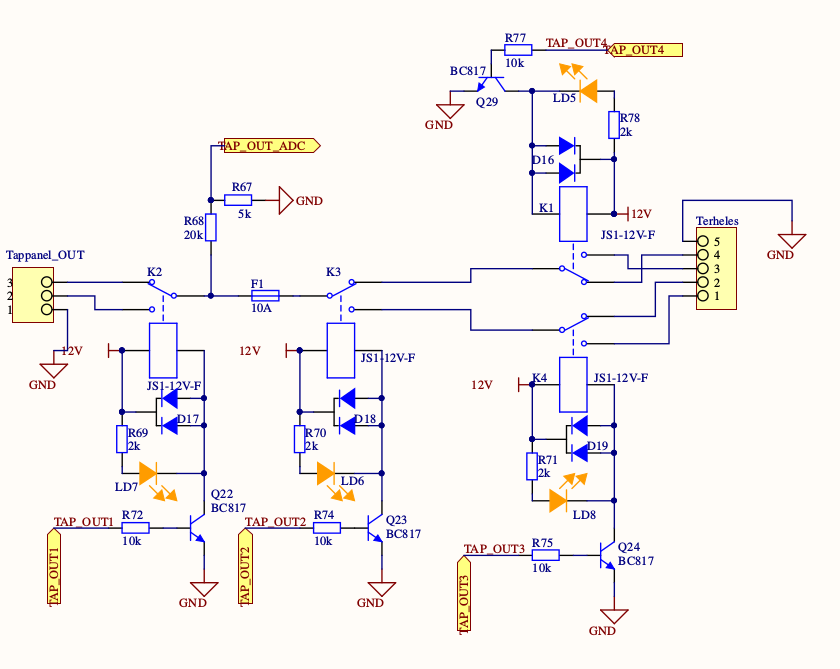
\includegraphics[clip, width=0.8\textwidth]{relays.png}}
    \caption{Táppanel terhelésének kapcsolása.}
\end{figure}

\subsubsection{Tápvonalakon rövidzárteszt}
Az ACU-n a 3.3V-os és a 12V-os vonalon is szeretnénk megnézni, hogy van-e rövidzár a GND felé, mielőtt bekapcsoljuk a készüléket. Ahhoz hogy ezeken a vonalakon mérni tudjam feszültséget kell kiadni rájuk, amitől viszont elindulna az eszköz, amit pedig nem szeretnénk. Ezért választottam azt a megoldást, hogy egy ellenálláson keresztül 3.3V-ra kapcsolom az egyik, majd a másik vonalat és közben AD átalakítóval nézem, hogy emelkedik-e a feszültségük. Ha rövidzár van a GND és a tápvonal között, akkor nem fog feszültség megjelenni az AD bemeneten. Az alábbi kapcsolás mutatja, hogy ezt hogyan valósítom meg. A diódára azért van szükség, hogy a teszter felé ne tudjon áram folyni. Bár ez megemeli a kezdeti feszültséget, amit érzékelni tudunk, de a kapcsolás emellett működőképes marad.
TODO kép

\subsection{Ethernet csatlakozó}
TODO pcb kialakítás, led jelek benne

\subsection{Egyéb}
TODO Biztosítékok, Felfogatás a négy sarkon, 0603-as alkatrészválasztás



\begin{figure}[H]
    \centering
	\fbox{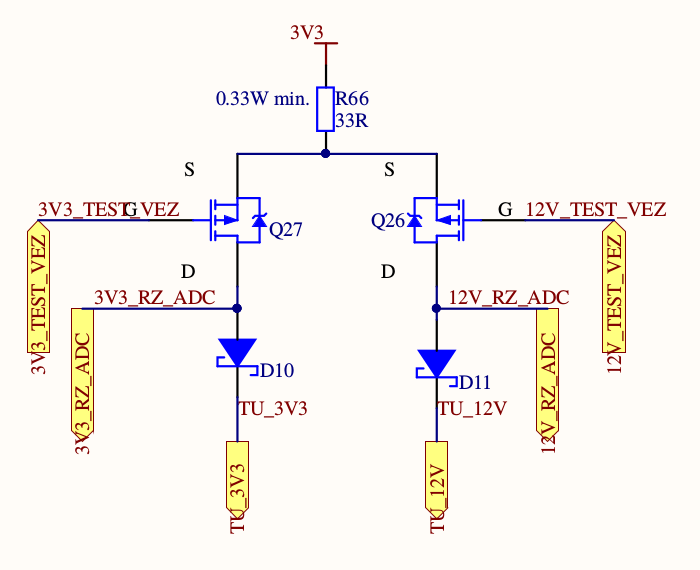
\includegraphics[clip, width=0.8\textwidth]{tapteszt.png}}
    \caption{Tápvonalak tesztelése.}
\end{figure}




\subsubsection{Programozás, kiegészítők}
\emph{ \tab A mikrokontrollerünk programozását JTAG-en keresztül végezzük, ehhez a megfelelő jeleket\footnote{$JTAG\ jelei:\ TDI,\ TDO,\ TMS,\ TCK,\ \overline{RST}$} IDC csatlakozón keresztül kivezettem.\\
2 nyomógombot és 3 ledet is terveztem a panelre, amelyeket tudunk bármire használni; a teszter firmware-ének ellenőrzését megkönnyíti, ha ilyen módon tudunk kommunikálni a panellel.\\
A mikrovezérlő órajelét egy 25MHz-es kristályoszcsillátor szolgáltatja. Bár van belső oszcillátora a mikrokontrollernek, az Ethernekhez szükséges a 25MHz-es oszcillátor és így nagyobb órajelről is tudjuk üzemeltetni az eszközünket.\\
A vezérlőegység időmérésének az alapja egy RTC, amit viszont kalibrálnunk kell minden egyes panelen. Ehhez tudunk olyan segítséget nyújtani, hogy ha jelezzük a vezérlőegység felé (például egy Ethernet csomaggal), hogy az egyik lábára érkező jel pontos 1Hz-es jel, akkor ő tudja magát kalibrálni. Ehhez egy olcsón beszerezhető GPS modult használunk, ami egy kész legyártott áramkör, aminek csak tápfeszültséget kell biztosítanunk és az másodpercenként impulzust generál, ehhez biztosítunk egy vonalat a panelünkön, valamint kivezetünk 3.3V-os tápfeszültséget is a GPS modulhoz. Ezzel az áramkörrel lehet kommunikálni UART kapcsolaton keresztül ezért egy TX és egy RX vonalat is kivezetünk és ha szükség lesz rá, akkor tudjuk használni.} A GPS modul rögzítésére a PCB terven középen az alsó harmadnál elhelyezkedő 4 furat és 5 pin szolgál.


\subsection{Kapcsolási rajz és PCB}
\tab Az eszköz tervezését az Altium\textregistered{} nevű programmal végeztem. A kapcsolási rajz elkészítése párhuzamosan zajlott a gondolkodással és tervezgetéssel, ezért többször is át kellett alakítani, ahogy jöttek az újabb és újabb ötletek, megvalósítási lehetőségek.\\
Szempont volt az is a tervezés során, hogy azokat az alkatrészeket, amik a cégben vannak lehessen használni, mert azzal már van tapasztalatunk és esetleg programmodulunk is. Egy ilyenre példa a flash memória, ugyanezt a típust használja egy másik panel is, ahol szintén ugyanaz a Texas Instrument által gyártott kontroller a központi egység, így ehhez már nem kell majd megírnunk a kommunikációs \emph{.h} fájlt, mert készen van, csak használnunk kell.\\
A PCB tervezésnél az általános szempontok mellett figyelembe vettem, hogy minél kisebb helyen elférjen a kapcsolás. Az önálló laboratóriumi munka utáni átalakításnál már nagyobb tapasztalattal tudtam ebbe belefogni és sikerült a korábbinál kisebb tervet készíteni, annak ellenére, hogy több helyet foglalnak az alkatrészek.

\section{Firmware}

\section{Értékelés, eredmények}
\tab Az első félév során elkészült kapcsolási rajz és PCB terv volt a célkitűzés, ami meg is valósult.A következő félévben a firmware írása és a kalibráció  a feladat. A firmware írásába is belefogtam, de ennek még nagyon az elején tartok.\\
Alább a teljes kapcsolási rajz és PCB terv látható.


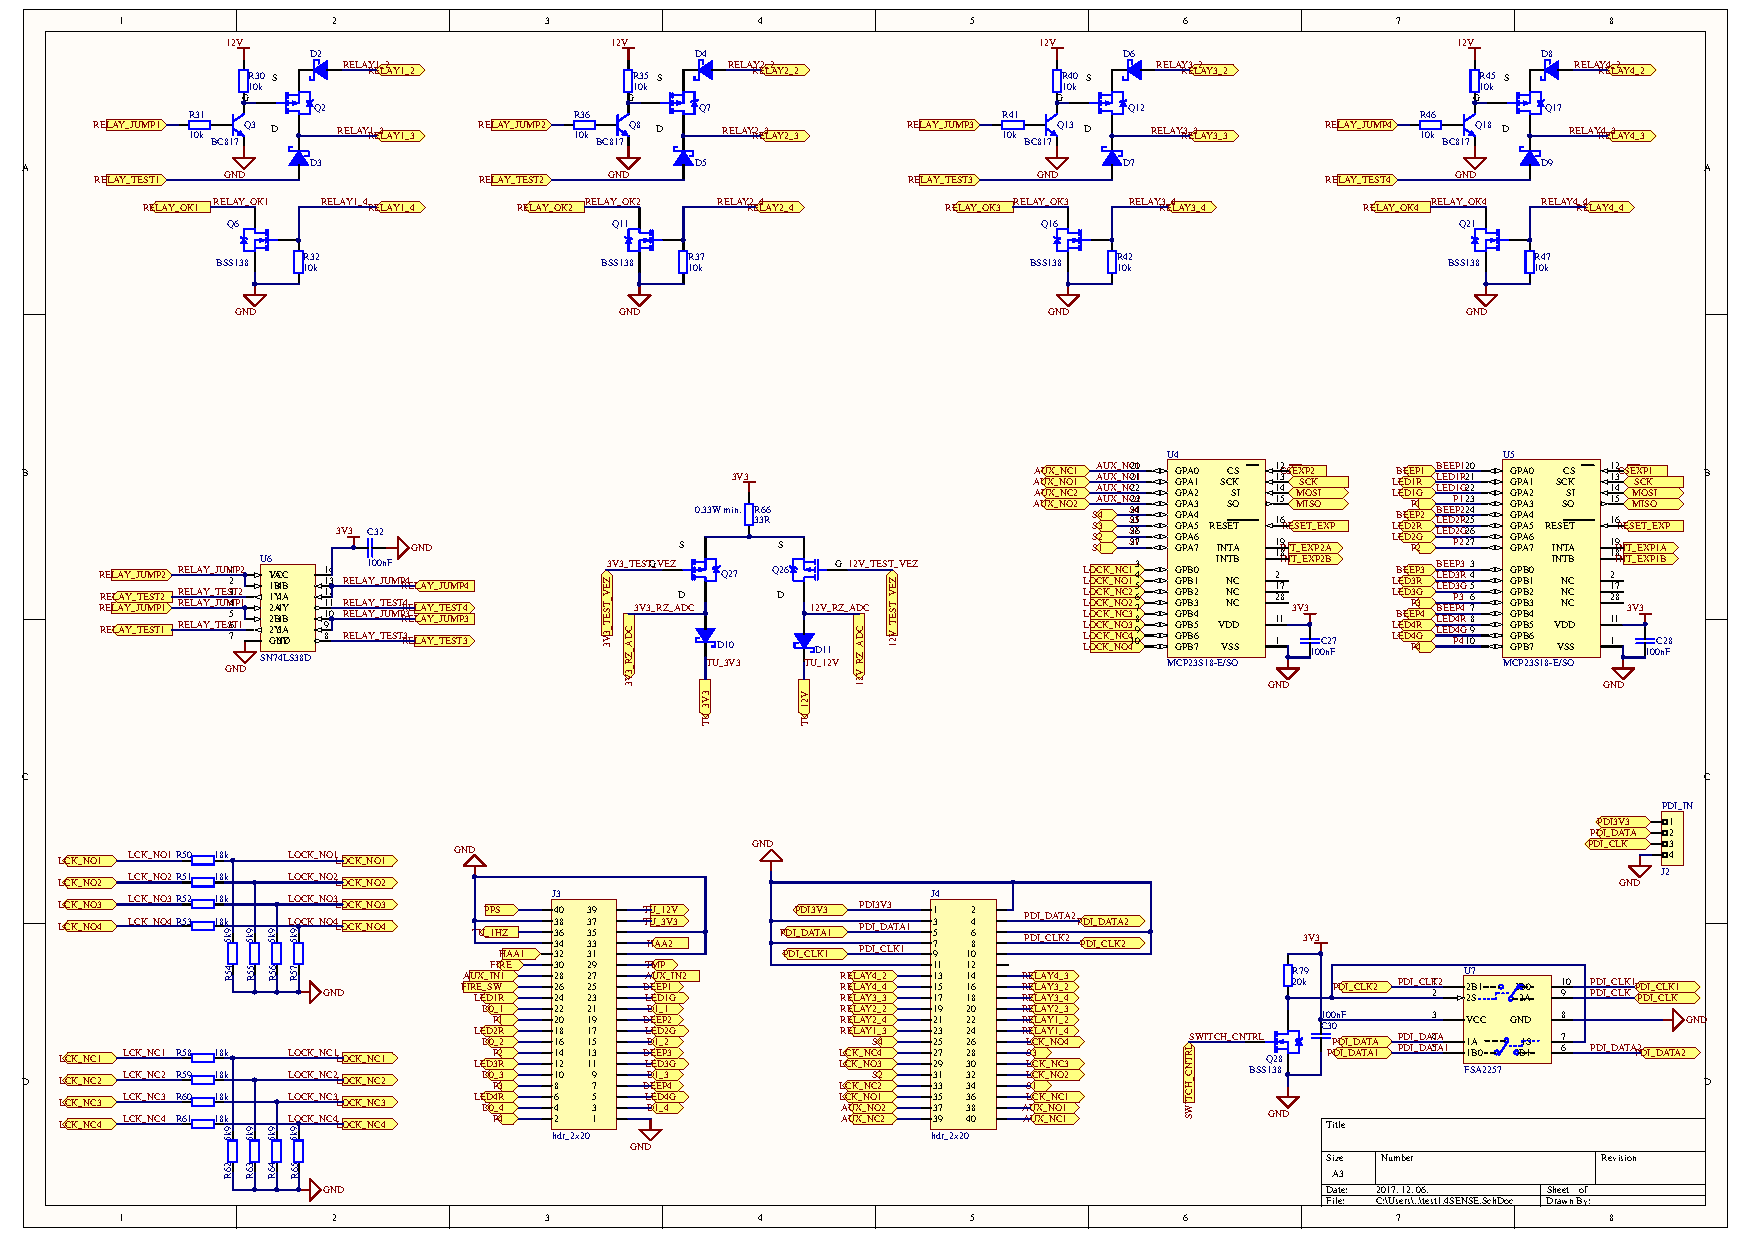
\includepdf[scale=0.78, angle=90]{test1pont41.pdf}
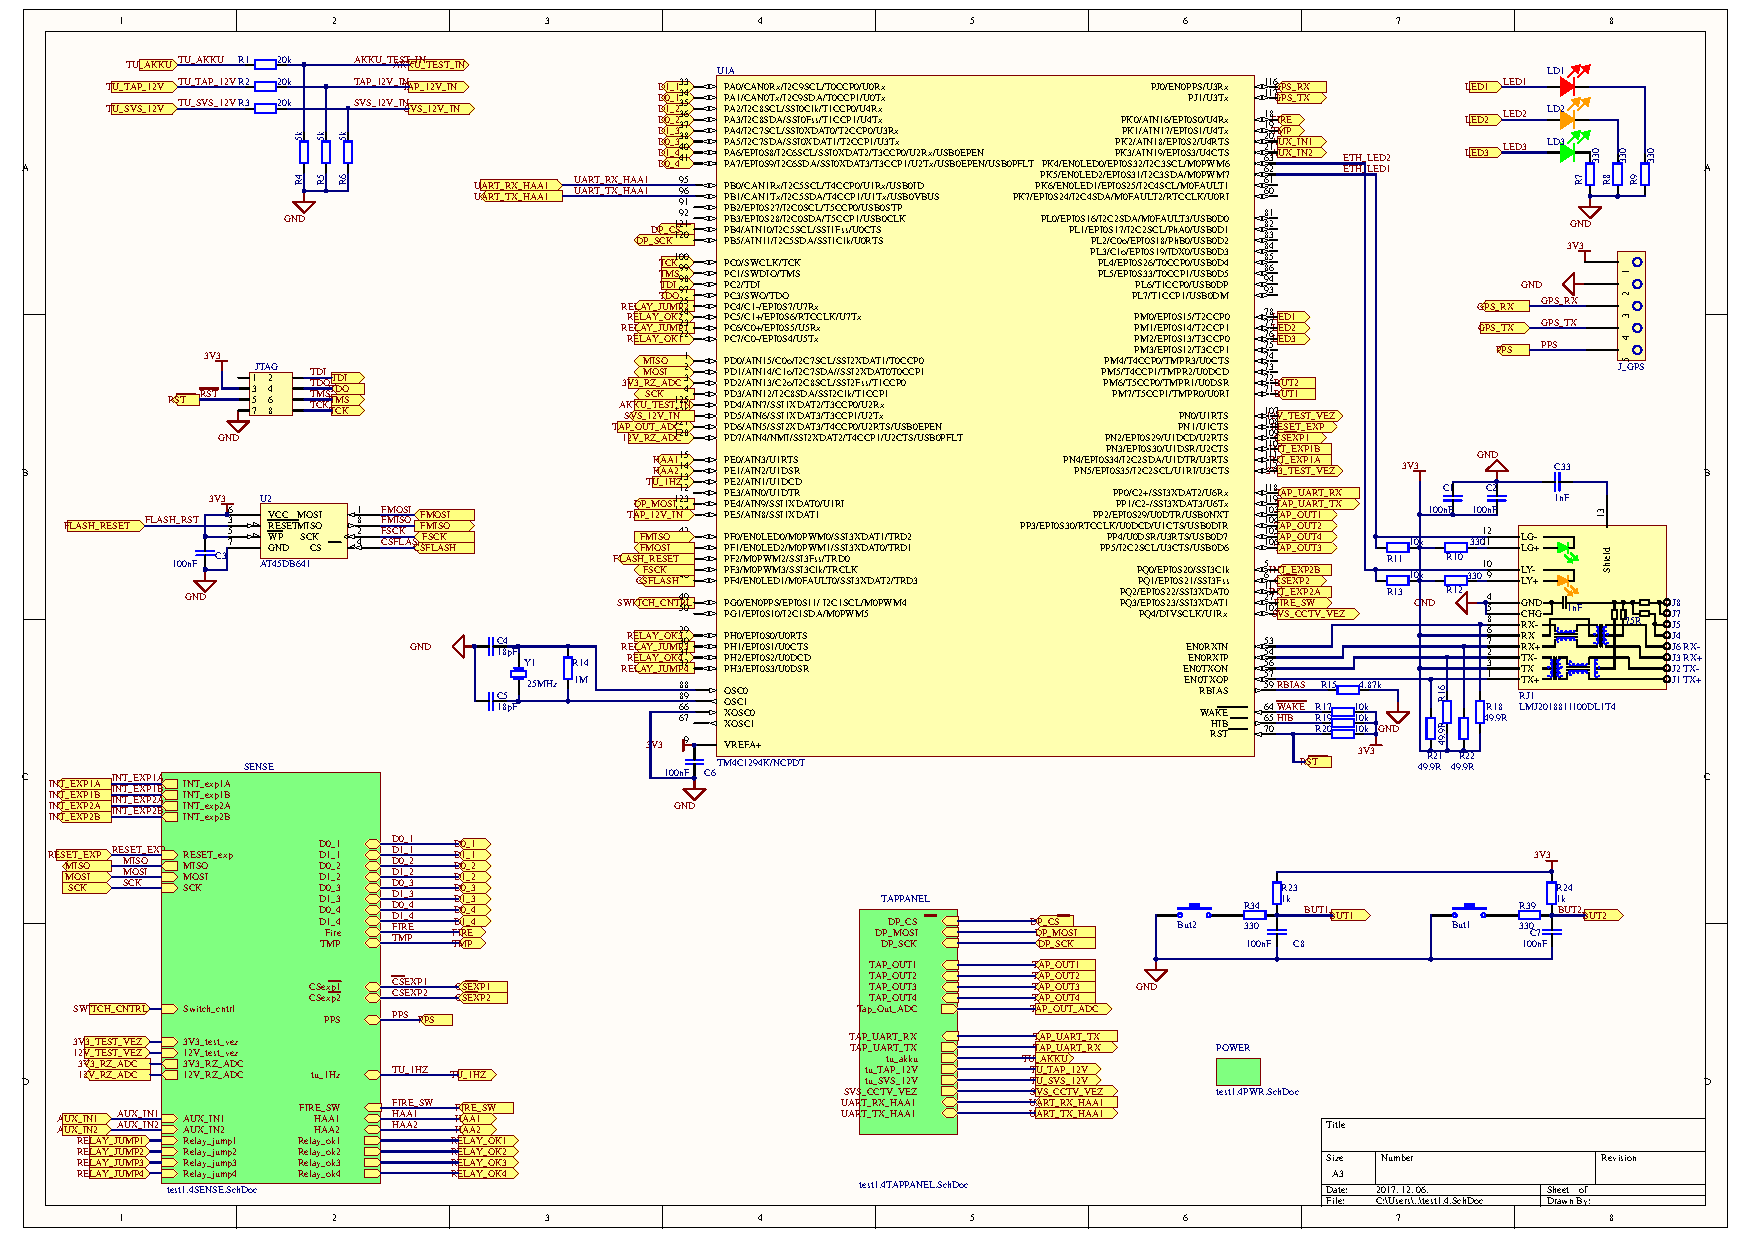
\includepdf[scale=0.78, angle=90]{test1pont42.pdf}
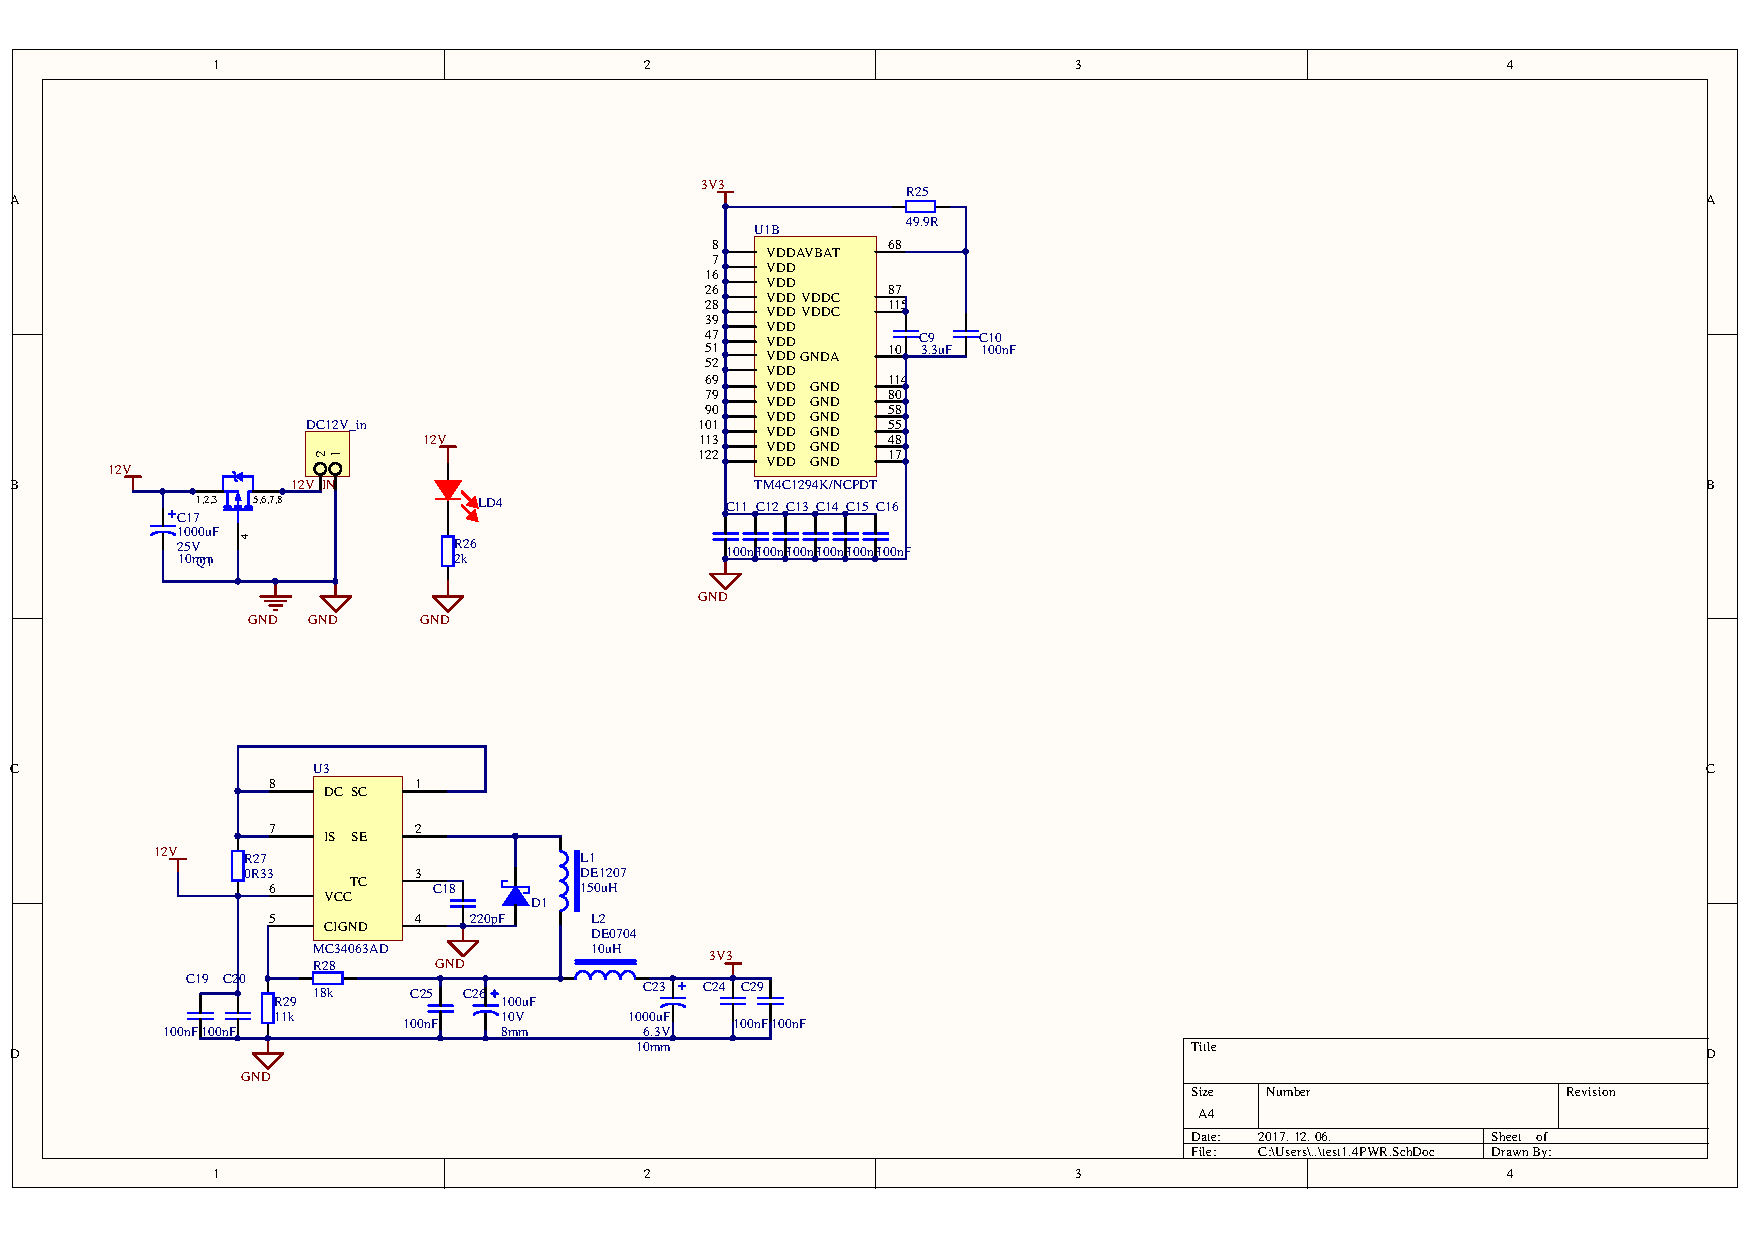
\includepdf[scale=0.78, angle=90]{test1pont43.pdf}
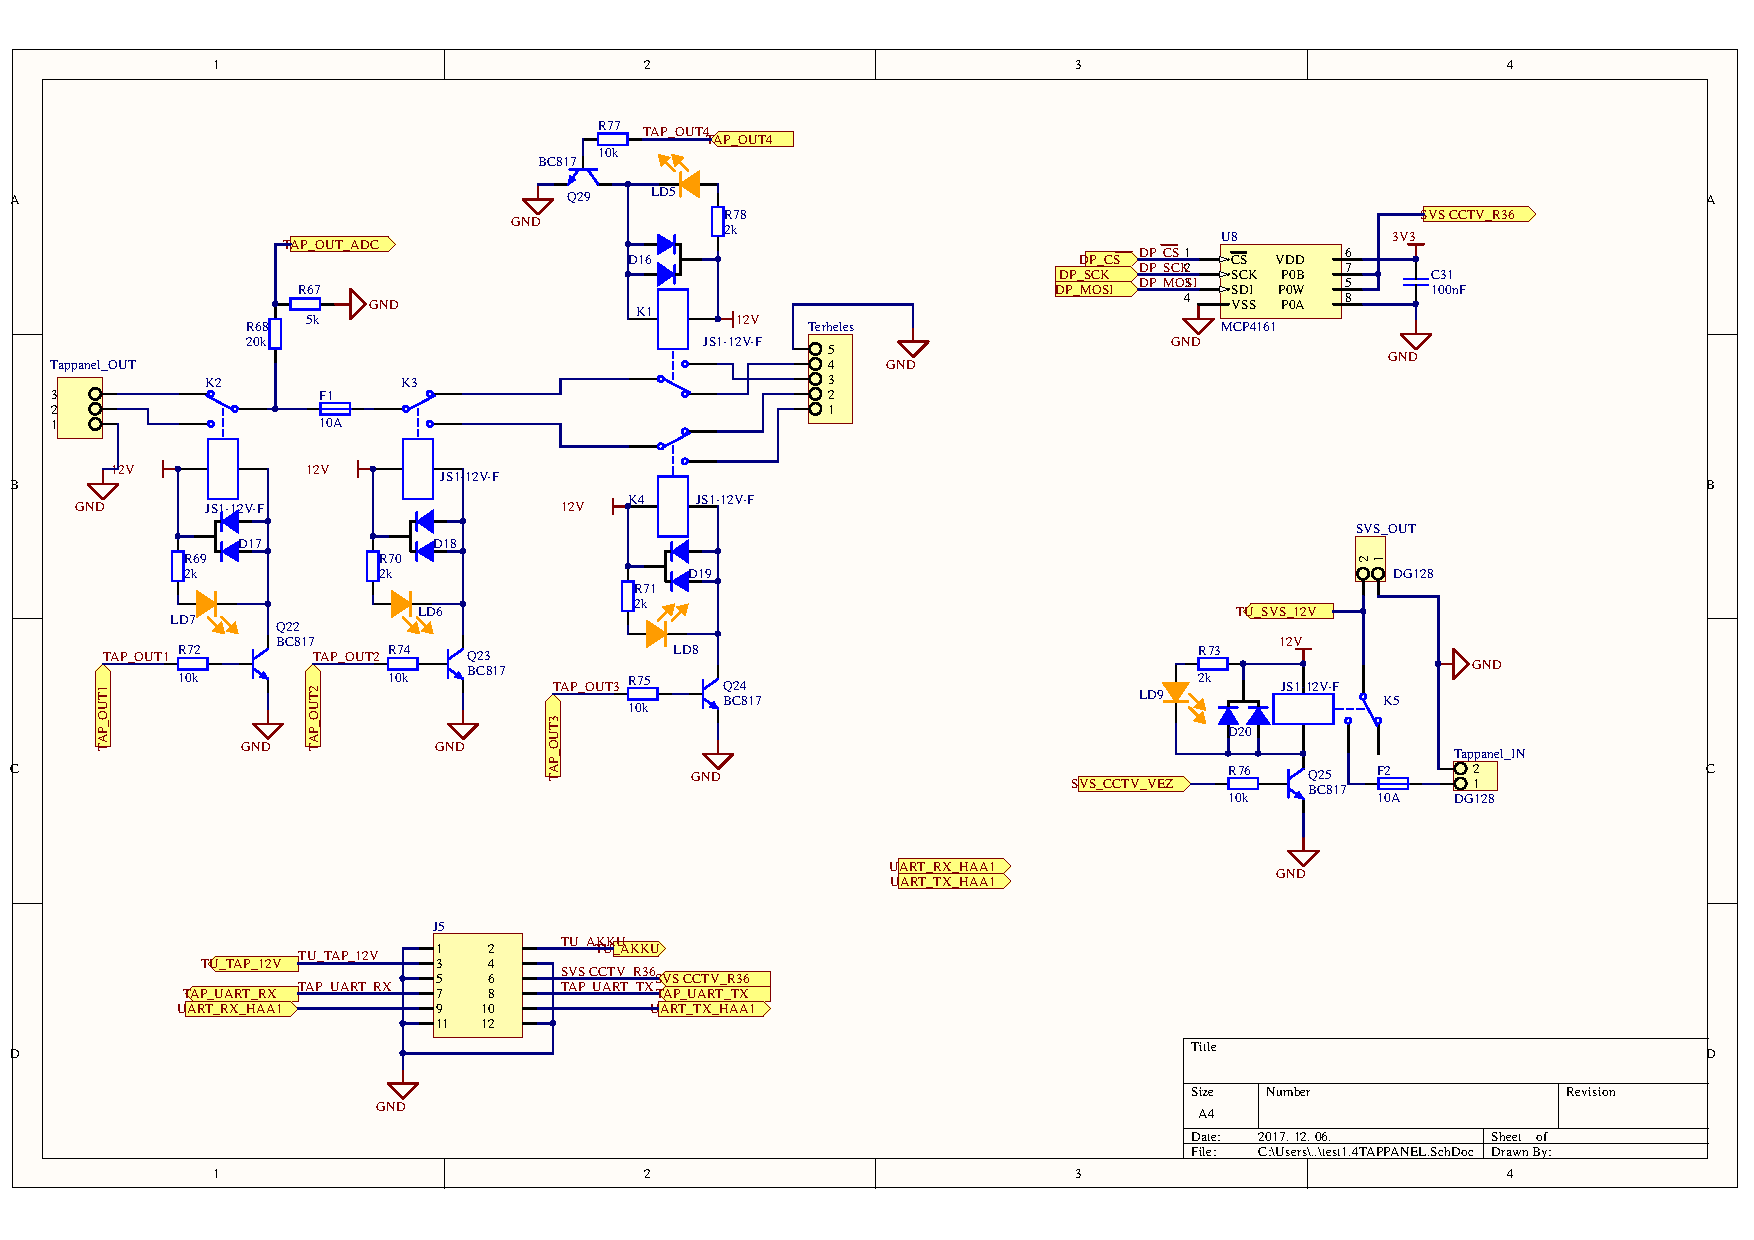
\includepdf[scale=0.78, angle=90]{test1pont44.pdf}
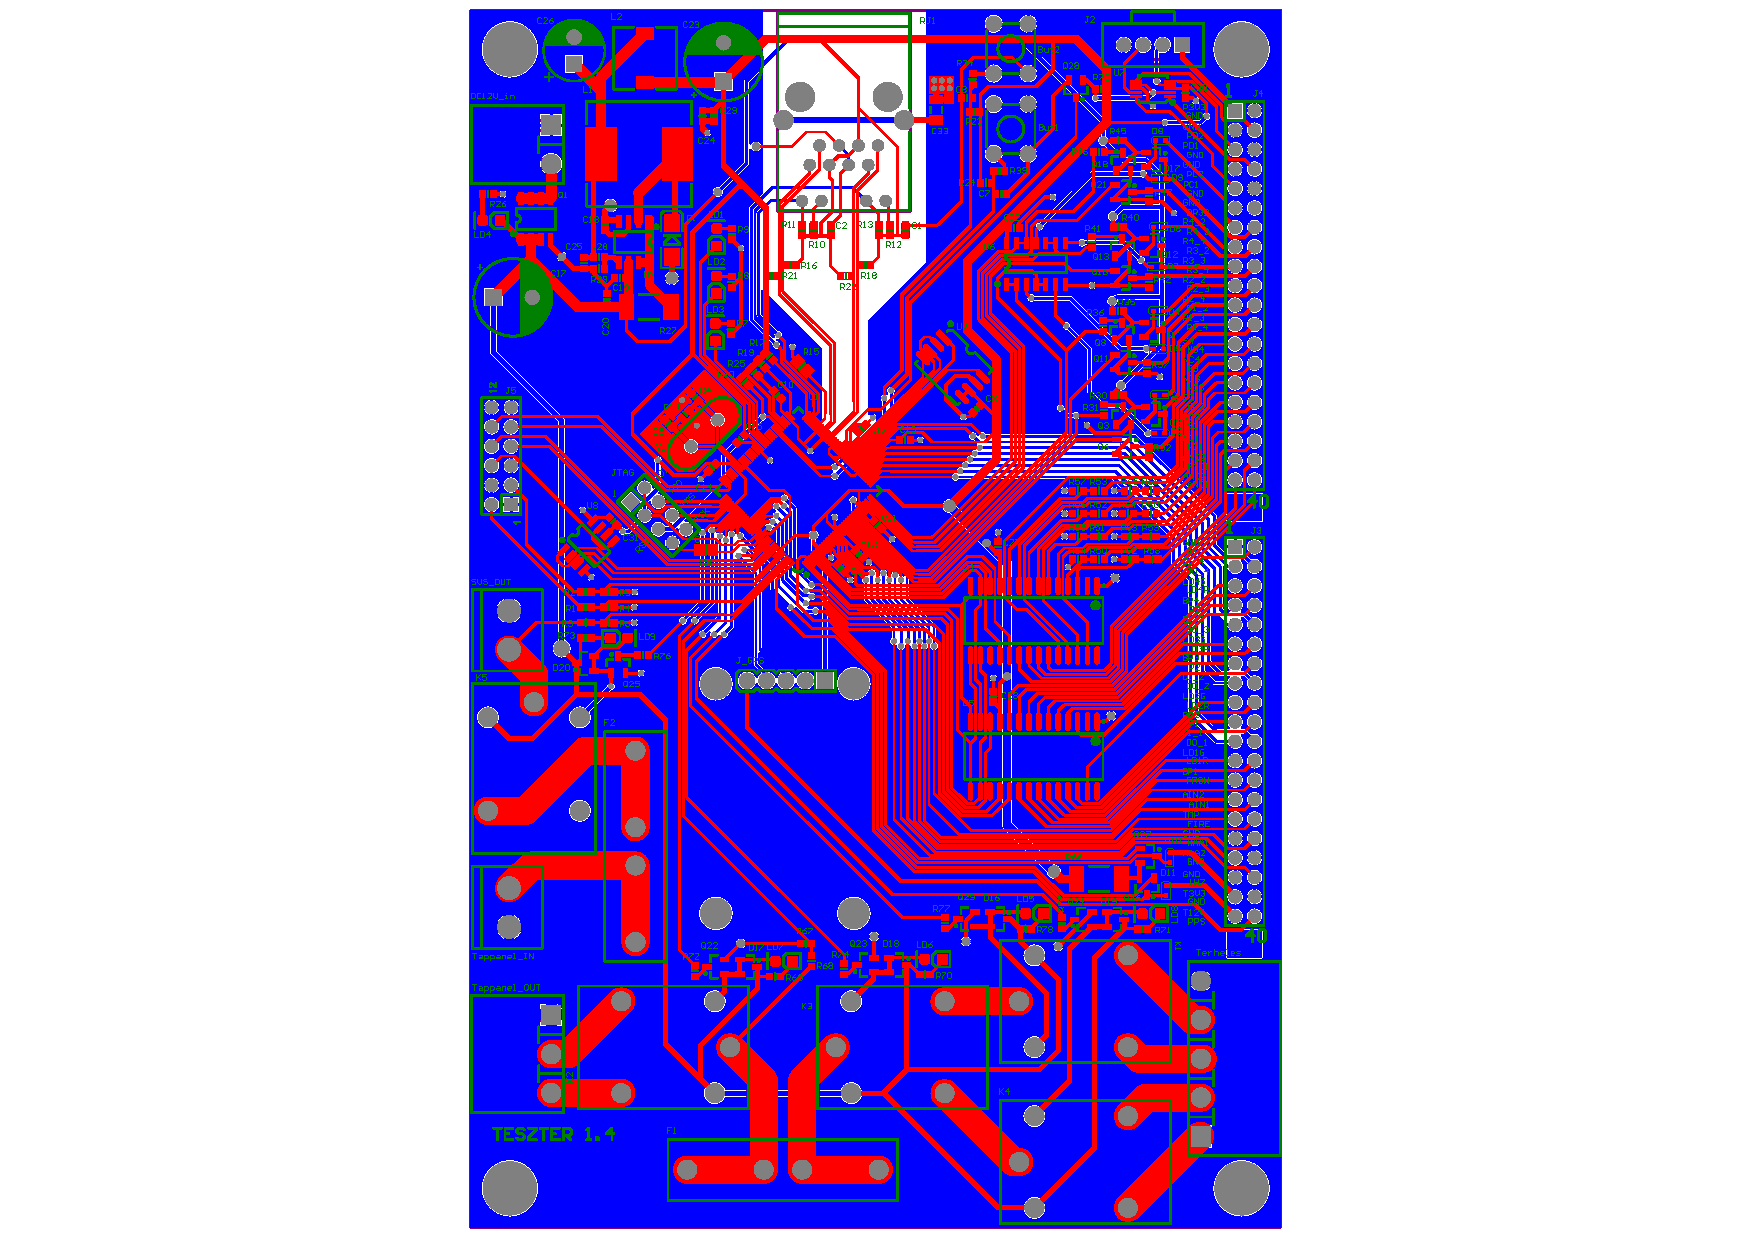
\includepdf[scale=1.6]{test1pont45.pdf}

\begin{figure}[H]
    \centering
	\fbox{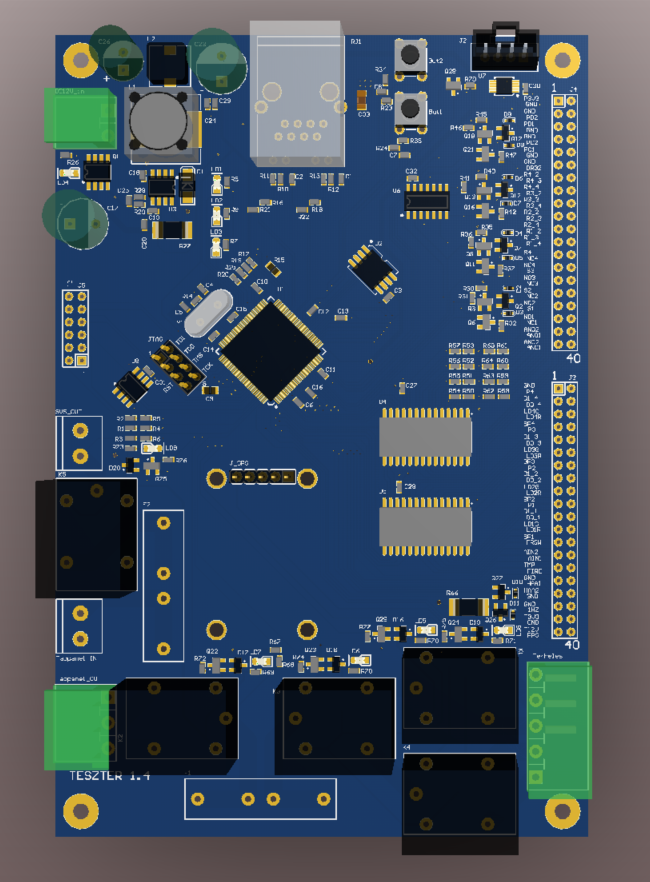
\includegraphics[clip]{3D.png}}
    \caption{Az eszköz 3 dimenziós képe.}
\end{figure}
\clearpage


\bibliographystyle{abbrv}
\bibliography{bib}
\vspace{1cm}

\end{document}